% =====================================================================
%  JUNA vs RPC -- Information-Theoretic Perspective
%  Beamer source, academic parchment style
%  Compile:  pdflatex JUNA_vs_RPC.tex   (run twice)
% =====================================================================
\documentclass[aspectratio=169,10pt]{beamer}

\usepackage[T1]{fontenc}
\usepackage{amsmath,amssymb,amsfonts}
\usepackage{bm}
\usepackage{tikz}
\usepackage{xcolor}
\usepackage{array}
\usepackage{booktabs}
\usepackage{colortbl}
\usepackage{etoolbox}
\usetikzlibrary{arrows.meta,positioning,shapes,fit,calc,backgrounds,decorations.pathreplacing}

% --------- color palette (parchment academic) ----------
\definecolor{parchment}{HTML}{F4E8C8}
\definecolor{paper}    {HTML}{FAF1D8}
\definecolor{ink}      {HTML}{1A1A1A}
\definecolor{inkgray}  {HTML}{5A5A5A}
\definecolor{rpcred}   {HTML}{8B1A1A}
\definecolor{junagreen}{HTML}{2D5F2C}
\definecolor{boxblue}  {HTML}{1F4E79}
\definecolor{redbg}    {HTML}{F7E0DE}
\definecolor{grnbg}    {HTML}{E0EBDC}
\definecolor{blubg}    {HTML}{DDE6EF}
\definecolor{labelbg}  {HTML}{EFE0B0}
\definecolor{headerbg} {HTML}{E8D9A8}

% --------- theme ----------
\usefonttheme{serif}
\setbeamercolor{background canvas}{bg=parchment}
\setbeamercolor{normal text}{fg=ink}
\setbeamercolor{structure}{fg=ink}
\setbeamercolor{frametitle}{fg=ink,bg=parchment}
\setbeamercolor{title}{fg=ink}
\setbeamercolor{itemize item}{fg=ink}
\setbeamercolor{itemize subitem}{fg=ink}
\setbeamercolor{item}{fg=ink}
\setbeamercolor{caption name}{fg=ink}
\setbeamertemplate{navigation symbols}{}
\setbeamertemplate{itemize item}{\textbullet}

% Frame title: centered bold serif with horizontal rule beneath
\setbeamertemplate{frametitle}{%
  \vspace{0.25em}%
  \begin{center}%
    {\bfseries\Large\insertframetitle\par}%
    \ifdefempty{\insertframesubtitle}{}{%
      \vspace{0.10em}{\itshape\normalsize\insertframesubtitle\par}%
    }%
    \vspace{0.30em}%
    {\color{ink}\rule{0.86\paperwidth}{0.4pt}}%
  \end{center}%
  \vspace{0.10em}%
}

% Footline: page number, italic, bottom-right
\setbeamertemplate{footline}{%
  \hbox to \paperwidth{\hfil\itshape\small\insertframenumber\hspace{0.7em}}%
  \vspace{0.35em}%
}

% --------- math shortcuts ----------
\newcommand{\vY}{\bm{Y}}
\newcommand{\vc}{\bm{c}}
\newcommand{\vn}{\bm{n}}
\newcommand{\vv}{\bm{v}}
\newcommand{\vH}{\bm{H}}
\newcommand{\vW}{\bm{W}}
\newcommand{\vX}{\bm{X}}
\newcommand{\vz}{\bm{z}}
\newcommand{\vC}{\bm{C}}
\newcommand{\vs}{\bm{s}}
\newcommand{\hvX}{\hat{\bm{X}}}
\newcommand{\hX}{\hat{X}}
\newcommand{\hb}{\hat{b}}
\newcommand{\herm}{\mathsf{H}}
\renewcommand{\Re}{\mathbb{R}}
\newcommand{\Cx}{\mathbb{C}}
\newcommand{\Bk}{\mathcal{B}_K(k)}

% --------- TikZ styles ----------
\tikzset{
  flowbox/.style   ={draw=ink, fill=paper, line width=0.6pt,
                     minimum width=2.5cm, minimum height=1.0cm,
                     align=center, font=\small\bfseries, inner sep=4pt},
  smallbox/.style  ={draw=ink, fill=paper, line width=0.4pt,
                     minimum width=0.7cm, minimum height=0.55cm,
                     inner sep=2pt, align=center, font=\footnotesize\itshape},
  branchbox/.style ={draw=ink, fill=paper, line width=0.4pt,
                     minimum width=2.0cm, minimum height=2.0cm,
                     inner sep=4pt, align=center, font=\footnotesize\itshape},
  flowarr/.style   ={-{Stealth[length=2.5mm,width=2mm]}, line width=0.7pt},
  redarr/.style    ={-{Stealth[length=2mm,width=1.6mm]}, line width=0.5pt, color=rpcred},
  rpcbox/.style    ={draw=rpcred,    line width=1.0pt, fill=paper,
                     align=center, font=\small\bfseries, inner sep=6pt},
  junabox/.style   ={draw=junagreen, line width=1.0pt, fill=paper,
                     align=center, font=\small\bfseries, inner sep=6pt},
  bluebox/.style   ={draw=boxblue,   line width=1.0pt, fill=paper,
                     align=center, font=\small\bfseries, inner sep=6pt},
}

% Standard inline label below a node label
\newcommand{\caplabel}[1]{{\footnotesize\itshape\color{inkgray}#1}}

% =====================================================================
\begin{document}

% =====================================================================
%  Slide 1: Title
% =====================================================================
\begin{frame}[plain]
  \vspace{1.3cm}
  \begin{center}
    {\bfseries\Huge JUNA vs Partial-FFT Combining:\par}
    \vspace{0.45em}
    {\bfseries\LARGE A FUNDAMENTAL DIFFERENCE\par}
    \vspace{0.30em}
    {\bfseries\LARGE IN WHAT IS ESTIMATED AND USED\par}

    \vspace{0.9cm}
    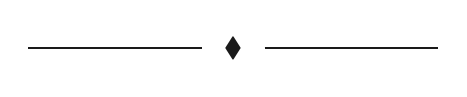
\begin{tikzpicture}
      \draw[ink,line width=0.5pt] (-2.6,0) -- (-0.4,0);
      \node at (0,0) {\color{ink}$\blacklozenge$};
      \draw[ink,line width=0.5pt] (0.4,0) -- (2.6,0);
    \end{tikzpicture}

    \vspace{0.7cm}
    {\Large Joint Unified Nonideality-Aware Algorithm (JUNA)\par}
    \vspace{0.15em}
    {\Large for Doppler-Resilient OFDM\par}

    \vspace{0.8cm}
    {\itshape\large\color{inkgray}--- Information-Theoretic Perspective ---\par}
    \vspace{0.25em}
    {\itshape\normalsize\color{inkgray}
      The comparison uses the Section II partial-FFT combining receiver\par}
  \end{center}
\end{frame}

% =====================================================================
%  Slide 2: System Model (Partial-FFT Domain)
% =====================================================================
\begin{frame}{1. System model}

  \begin{columns}[T,onlytextwidth]
    \begin{column}{0.46\textwidth}
      \begin{itemize}\setlength{\itemsep}{0.5em}
        \item Residual Doppler causes intercarrier interference (ICI)
        \item Each carrier depends on nearby transmitted symbols
        \item Partial FFT gives $M$ branches per carrier
      \end{itemize}
    \end{column}
    \begin{column}{0.52\textwidth}
      For received carrier $k$:
      \vspace{-0.2em}
      \[
        \vY_k \;=\;
        \sum_{q\in\Bk}\;
        \underbrace{\vc_{k,q}}_{\substack{\text{\scriptsize branch-domain}\\\text{\scriptsize coefficient vector}\\\text{\scriptsize $(M\times 1)$}}}\;
        \underbrace{s_q}_{\substack{\text{\scriptsize transmitted}\\\text{\scriptsize symbol}}}\;+\;
        \underbrace{\vn_k}_{\substack{\text{\scriptsize noise}\\\text{\scriptsize vector}}}
      \]
    \end{column}
  \end{columns}

  \vspace{0.5em}
  \begin{itemize}\setlength{\itemsep}{0.2em}
    \item $\vY_{k}\in\Cx^{M\times 1}$ : partial-FFT observation at carrier $k$
    \item $\vc_{k,q}\in\Cx^{M\times 1}$ : local ICI / nonideality coefficient from $q\to k$
  \end{itemize}

  \vspace{0.4em}
  \begin{center}
  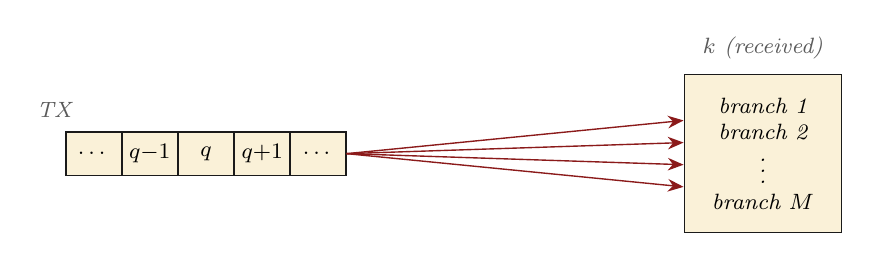
\begin{tikzpicture}[node distance=0pt]
    \node[font=\footnotesize\itshape\color{inkgray}] at (-0.5,0.55) {TX};
    \node[smallbox] (s1) at (0.0,0)   {$\dots$};
    \node[smallbox,right=0pt of s1] (s2) {$q{-}1$};
    \node[smallbox,right=0pt of s2] (s3) {$q$};
    \node[smallbox,right=0pt of s3] (s4) {$q{+}1$};
    \node[smallbox,right=0pt of s4] (s5) {$\dots$};

    \node[branchbox] (br) at (8.5,0) {branch 1\\branch 2\\$\vdots$\\branch $M$};
    \node[font=\footnotesize\itshape\color{inkgray},above=2pt of br]
      {$k$ (received)};

    \draw[redarr] (s5.east) -- ([yshift=12pt]br.west);
    \draw[redarr] (s5.east) -- ([yshift=4pt]br.west);
    \draw[redarr] (s5.east) -- ([yshift=-4pt]br.west);
    \draw[redarr] (s5.east) -- ([yshift=-12pt]br.west);
  \end{tikzpicture}
  \end{center}
\end{frame}

% =====================================================================
%  Slide 3: Where Doppler Enters
% =====================================================================
\begin{frame}{2. Doppler and ICI}

  \begin{columns}[T,onlytextwidth]
    \begin{column}{0.47\textwidth}
      \begin{itemize}\setlength{\itemsep}{0.42em}
        \item Full FFT demodulates carrier $k$ over the symbol:
              \[
                y_k=\frac{1}{\sqrt{T}}\int_0^T r(t)e^{-j2\pi f_k t}\,dt .
              \]
        \item Static channel: orthogonality leaves $d_kH_k$ plus noise
        \item Doppler varies $H_i(t)$ inside the integral
        \item Hence the $i\ne k$ terms no longer cancel
      \end{itemize}
    \end{column}
    \begin{column}{0.51\textwidth}
      \begin{center}
      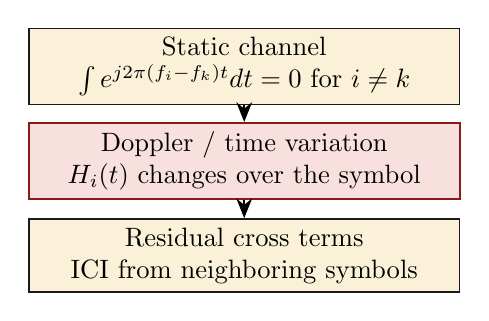
\begin{tikzpicture}[x=1cm,y=1cm,scale=0.96,every node/.style={transform shape}]
        \node[draw=ink,fill=paper,line width=0.6pt,
              minimum width=5.7cm,minimum height=0.9cm,align=center] (static) at (0,1.25)
          {Static channel\\$\int e^{j2\pi(f_i-f_k)t}dt=0$ for $i\ne k$};
        \node[draw=rpcred,fill=redbg,line width=0.8pt,
              minimum width=5.7cm,minimum height=0.9cm,align=center] (dop) at (0,0)
          {Doppler / time variation\\$H_i(t)$ changes over the symbol};
        \node[draw=ink,fill=paper,line width=0.6pt,
              minimum width=5.7cm,minimum height=0.9cm,align=center] (ici) at (0,-1.25)
          {Residual cross terms\\ICI from neighboring symbols};
        \draw[flowarr] (static.south) -- (dop.north);
        \draw[flowarr] (dop.south) -- (ici.north);
      \end{tikzpicture}
      \end{center}
    \end{column}
  \end{columns}

  \vfill
  \begin{center}
    
\begin{tikzpicture}
      \node[draw=ink,line width=0.6pt,fill=paper,
            minimum width=13.8cm,minimum height=1.0cm,
            align=center,inner sep=6pt]
        {Full-FFT OFDM assumes orthogonal tones over the whole symbol.\\
         Doppler time variation breaks that orthogonality and creates ICI.};
    \end{tikzpicture}
  \end{center}

\end{frame}

% =====================================================================
%  Slide 4: RPC as Section II Partial FFT
% =====================================================================
\begin{frame}{3. Partial-FFT combining}

  \begin{columns}[T,onlytextwidth]
    \begin{column}{0.48\textwidth}
      \begin{itemize}\setlength{\itemsep}{0.35em}
        \item Divide the symbol into $M$ non-overlapping windows
        \item FFT each short window:
              \[
                y_k(m)=\frac{1}{\sqrt{T}}
                \int_{\frac{m-1}{M}T}^{\frac{m}{M}T}
                r(t)e^{-j2\pi f_k t}\,dt .
              \]
        \item Approximate the channel by its midpoint value
      \end{itemize}
    \end{column}
    \begin{column}{0.50\textwidth}
      \[
        \vY_k =
        \begin{bmatrix}
        y_k(1)\\ y_k(2)\\ \vdots\\ y_k(M)
        \end{bmatrix}
      \]
      \[
        \vY_k
        =
        \sum_i d_i\,\vH_i\,\vv_{i,k}+\vn_k
      \]
      \[
        \hX_k=\vW_k^{\herm}\vY_k
      \]
    \end{column}
  \end{columns}

  \vspace{-0.3em}
  \begin{center}
  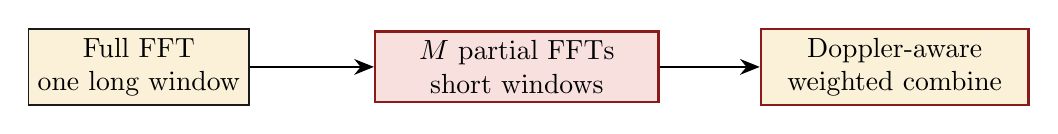
\begin{tikzpicture}[x=1cm,y=1cm]
    \node[draw=ink,fill=paper,line width=0.6pt,
          minimum width=2.6cm,minimum height=0.9cm,align=center] (full) at (-4.8,0)
      {Full FFT\\one long window};
    \node[draw=rpcred,fill=redbg,line width=0.8pt,
          minimum width=3.6cm,minimum height=0.9cm,align=center] (parts) at (0,0)
      {$M$ partial FFTs\\short windows};
    \node[draw=rpcred,fill=paper,line width=0.8pt,
          minimum width=3.4cm,minimum height=0.9cm,align=center] (comb) at (4.8,0)
      {Doppler-aware\\weighted combine};
    \draw[flowarr] (full.east) -- (parts.west);
    \draw[flowarr] (parts.east) -- (comb.west);
  \end{tikzpicture}
  \end{center}

  \vfill
  \begin{center}
    
\begin{tikzpicture}
      \node[draw=ink,line width=0.6pt,fill=paper,
            minimum width=13.8cm,minimum height=1.0cm,
            align=center,inner sep=6pt]
        {The weights act like a carrier-specific stepwise receiver window.\\
         Hence the desired carrier adds more coherently and ICI is reduced.};
    \end{tikzpicture}
  \end{center}

\end{frame}

% =====================================================================
%  Slide 4a: Where the Partial-FFT Vector Model Comes From
% =====================================================================
\begin{frame}{3a. The branch model}

  \footnotesize
  \setlength{\abovedisplayskip}{0.35em}
  \setlength{\belowdisplayskip}{0.35em}
  \newcommand{\am}{a_m}
  \newcommand{\bmint}{b_m}
  \begin{columns}[T,onlytextwidth]
    \begin{column}{0.60\textwidth}
      Let $\am=\frac{m-1}{M}T$ and $\bmint=\frac{m}{M}T$.  After cyclic-prefix removal,
      \[
        r(t) \approx \frac{1}{\sqrt{T}}
        \sum_i d_i\,H_i(t)e^{j2\pi f_i t}+n(t).
      \]
      The $m$th partial FFT for bin $k$ gives
      \[
      \begin{aligned}
        y_k(m)
        &=\frac{1}{\sqrt{T}}\int_{\am}^{\bmint}
          r(t)e^{-j2\pi f_k t}\,dt\\
        &=\sum_i d_i\frac{1}{T}\int_{\am}^{\bmint}
          H_i(t)e^{j2\pi(f_i-f_k)t}\,dt+n_k(m)\\
        &\approx
        \sum_i d_i\,H_i(m)\,v_{i,k}(m)+n_k(m).
      \end{aligned}
      \]
      The last line is the midpoint approximation:
      $H_i(t)\approx H_i(m)$ inside the short interval.
    \end{column}

    \begin{column}{0.38\textwidth}
      \[
        v_{i,k}(m)=
        \frac{1}{T}\int_{\am}^{\bmint}
        e^{j2\pi(f_i-f_k)t}\,dt .
      \]
      Stack over all $M$ windows:
      \[
        \vY_k=[y_k(1),\ldots,y_k(M)]^{\mathsf T},
      \]
      \[
        \vv_{i,k}=[v_{i,k}(1),\ldots,v_{i,k}(M)]^{\mathsf T},
      \]
      \[
        \vH_i=\operatorname{diag}\{H_i(1),\ldots,H_i(M)\}.
      \]
      \vspace{0.2em}
      \[
        \Rightarrow\quad
        \boxed{
        \vY_k=\sum_i d_i\,\vH_i\,\vv_{i,k}+\vn_k
        }
      \]
    \end{column}
  \end{columns}

  \vspace{0.2em}
  \begin{center}
    {\itshape\footnotesize Source: Yerramalli, Stojanovic, and Mitra,
    IEEE TSP 2012, Sec. II-C, Eqs. (5)--(9). Their $\vv_{i-k}$ is written here as $\vv_{i,k}$.}
  \end{center}

\end{frame}

% =====================================================================
%  Slide 5: RPC vs JUNA (High-Level View)
% =====================================================================
\begin{frame}{4. Two receivers}

  \begin{center}
  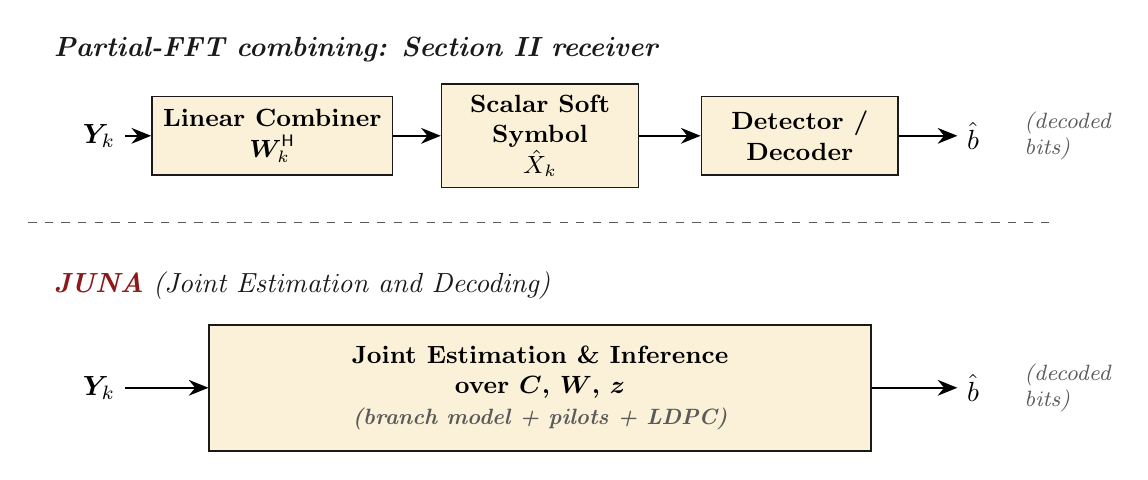
\begin{tikzpicture}[x=1cm,y=1cm]
    % RPC label
    \node[anchor=west,font=\itshape\bfseries\color{ink}] at (-6.3,2.6)
      {Partial-FFT combining: Section II receiver};

    \node                         (yk)  at (-5.6,1.5) {$\vY_k$};
    \node[flowbox]                (lc)  at (-3.4,1.5) {Linear Combiner\\$\vW_k^{\herm}$};
    \node[flowbox]                (ss)  at ( 0.0,1.5) {Scalar Soft\\Symbol\\$\hX_k$};
    \node[flowbox]                (ld)  at ( 3.3,1.5) {Detector /\\Decoder};
    \node                         (bh)  at ( 5.5,1.5) {$\hb$};
    \node[font=\footnotesize\itshape\color{inkgray},align=left] at (6.7,1.5) {(decoded\\bits)};

    \draw[flowarr] (yk.east) -- (lc.west);
    \draw[flowarr] (lc.east) -- (ss.west);
    \draw[flowarr] (ss.east) -- (ld.west);
    \draw[flowarr] (ld.east) -- (bh.west);

    % dashed separator
    \draw[dashed,color=inkgray] (-6.5,0.4) -- (6.5,0.4);

    % JUNA label
    \node[anchor=west] at (-6.3,-0.4)
      {{\itshape\bfseries\color{rpcred}JUNA} {\itshape\color{ink}(Joint Estimation and Decoding)}};

    \node                         (yk2) at (-5.6,-1.7) {$\vY_k$};
    \node[flowbox,minimum width=8.4cm,minimum height=1.6cm]
                                   (jb)  at ( 0.0,-1.7) {Joint Estimation \& Inference\\
                                                          over $\vC$, $\vW$, $\vz$\\
                                                          {\footnotesize\itshape\color{inkgray}(branch model + pilots + LDPC)}};
    \node                         (bh2) at ( 5.5,-1.7) {$\hb$};
    \node[font=\footnotesize\itshape\color{inkgray},align=left] at (6.7,-1.7) {(decoded\\bits)};

    \draw[flowarr] (yk2.east) -- (jb.west);
    \draw[flowarr] (jb.east)  -- (bh2.west);
  \end{tikzpicture}
  \end{center}

\end{frame}

% =====================================================================
%  Slide 6: RPC: What Is Used?
% =====================================================================
\begin{frame}{5. The combining weight}
  \begin{columns}[T,onlytextwidth]
    \begin{column}{0.46\textwidth}
      \begin{itemize}\setlength{\itemsep}{0.35em}
        \item Front end: partial-FFT observations, weighted combining
        \item Chosen to compensate time variation, reduce ICI
        \item Main quantity in the Section II construction:
      \end{itemize}

      \vspace{0.25em}
      \begin{center}
        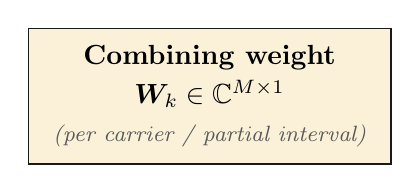
\begin{tikzpicture}
          \node[draw=ink,line width=0.6pt,fill=paper,
                minimum width=4.6cm,minimum height=1.6cm,
                align=center,inner sep=6pt] {%
            \textbf{Combining weight}\\[2pt]
            $\vW_k\in\Cx^{M\times 1}$\\[2pt]
            {\footnotesize\itshape\color{inkgray}(per carrier / partial interval)}};
        \end{tikzpicture}
      \end{center}
    \end{column}

    \begin{column}{0.52\textwidth}
      \begin{center}
      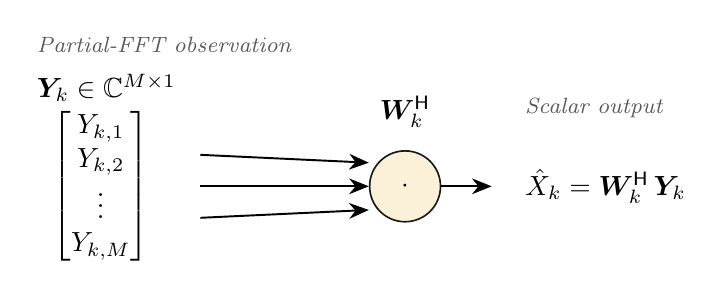
\begin{tikzpicture}[x=1cm,y=1cm]
        \node[font=\footnotesize\itshape\color{inkgray},anchor=west] at (-3.2,1.4)
          {Partial-FFT observation};
        \node[anchor=west] at (-3.2,0.85) {$\vY_k\in\Cx^{M\times 1}$};

        % Vector
        \node[anchor=west] at (-3.0,-0.4) {$\begin{bmatrix} Y_{k,1}\\ Y_{k,2}\\ \vdots\\ Y_{k,M}\end{bmatrix}$};

        % combiner
        \node[font=\bfseries] at (1.6,0.55) {$\vW_k^{\herm}$};
        \node[draw=ink,fill=paper,circle,inner sep=0pt,minimum size=0.9cm,line width=0.6pt] (cir) at (1.6,-0.4) {$\cdot$};

        % arrows in
        \draw[flowarr] (-1.0,0.0) -- ($(cir.west)+(0,0.3)$);
        \draw[flowarr] (-1.0,-0.4) -- (cir.west);
        \draw[flowarr] (-1.0,-0.8) -- ($(cir.west)+(0,-0.3)$);

        % arrow out
        \draw[flowarr] (cir.east) -- (2.7,-0.4);

        \node[font=\footnotesize\itshape\color{inkgray},anchor=west] at (3.0,0.6) {Scalar output};
        \node[anchor=west] at (3.0,-0.4) {$\hX_k = \vW_k^{\herm}\,\vY_k$};
      \end{tikzpicture}
      \end{center}
    \end{column}
  \end{columns}

  \vspace{0.15em}
  \begin{center}
    {\itshape\small While the combiner reduces ICI, it does not model the coded
    symbols jointly. Scalar combining maps the branch vector to one number
    before decoding.}
  \end{center}
\end{frame}

% =====================================================================
%  Slide 6a: How RPC Helps With Doppler
% =====================================================================
\begin{frame}{5a. Doppler compensation}

  \footnotesize
  \setlength{\abovedisplayskip}{0.45em}
  \setlength{\belowdisplayskip}{0.45em}
  \begin{columns}[T,onlytextwidth]
    \begin{column}{0.52\textwidth}
      \begin{itemize}\setlength{\itemsep}{0.25em}
        \item Channel varies inside the symbol; the FFT mixes carriers
        \item Partial FFT turns time variation into $M$ branches:
              \[
	                H_i(t)\quad\leadsto\quad
	                \big[H_i(1),\ldots,H_i(M)\big].
	              \]
        \item Branch differences are the degrees of freedom
        \item Align the desired carrier, reduce nearby ICI
      \end{itemize}

      \vspace{-0.15em}
      \begin{center}
      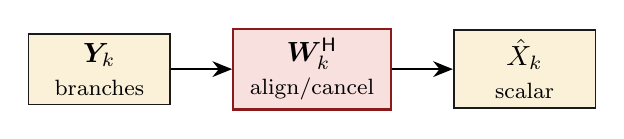
\begin{tikzpicture}[x=1cm,y=1cm]
        \node[draw=ink,fill=paper,line width=0.6pt,
              minimum width=1.8cm,minimum height=0.65cm,align=center] (branch) at (-2.7,0)
          {$\vY_k$\\{\footnotesize branches}};
        \node[draw=rpcred,fill=redbg,line width=0.8pt,
              minimum width=2.0cm,minimum height=0.65cm,align=center] (w) at (0.0,0)
          {$\vW_k^{\herm}$\\{\footnotesize align/cancel}};
        \node[draw=ink,fill=paper,line width=0.6pt,
              minimum width=1.8cm,minimum height=0.65cm,align=center] (out) at (2.7,0)
          {$\hX_k$\\{\footnotesize scalar}};
        \draw[flowarr] (branch.east) -- (w.west);
        \draw[flowarr] (w.east) -- (out.west);
      \end{tikzpicture}
      \end{center}
    \end{column}

    \begin{column}{0.46\textwidth}
      \vspace{-0.6em}
      \[
      \begin{gathered}
        \vc_{i,k}=\vH_i\vv_{i,k},\qquad
        a_{i,k}=\vW_k^{\herm}\vc_{i,k},\\[-1pt]
        \tilde n_k=\vW_k^{\herm}\vn_k .
      \end{gathered}
      \]
      \vspace{-0.7em}
      \[
      \begin{aligned}
        \hX_k
        &=\vW_k^{\herm}\vY_k\\
        &=d_k a_{k,k}
          +\sum_{i\ne k} d_i a_{i,k}
          +\tilde n_k\\
        &\approx d_k+\tilde n_k .
      \end{aligned}
      \]

      \vspace{-0.6em}
      \[
        a_{k,k}\approx 1,
        \qquad
        a_{i,k}\approx 0
        \quad (i\ne k \text{ nearby}).
      \]

      \vspace{-0.1em}
      \begin{center}
        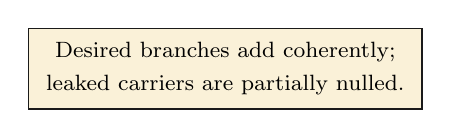
\begin{tikzpicture}
          \node[draw=ink,line width=0.6pt,fill=paper,
                minimum width=5.0cm,minimum height=0.85cm,
                align=center,inner sep=5pt]
            {\footnotesize Desired branches add coherently;\\
             \footnotesize leaked carriers are partially nulled.};
        \end{tikzpicture}
      \end{center}
    \end{column}
  \end{columns}

  \vspace{0.2em}
  \begin{center}
    {\itshape\footnotesize While the combiner builds a Doppler-compensated
    observation for each carrier, it does not estimate the coded symbols jointly.}
  \end{center}

\end{frame}

% =====================================================================
%  Slide 6b: Branch Projection Diagram
% =====================================================================
\begin{frame}{5b. Branch projection}

  \small
  \setlength{\abovedisplayskip}{0.35em}
  \setlength{\belowdisplayskip}{0.35em}
  \[
    \vc_{i,k}\equiv \vH_i\vv_{i,k},
    \qquad
    \vY_k=d_k\vc_{k,k}+\sum_{i\ne k}d_i\vc_{i,k}+\vn_k .
  \]

  \vspace{-0.6em}
  \begin{center}
  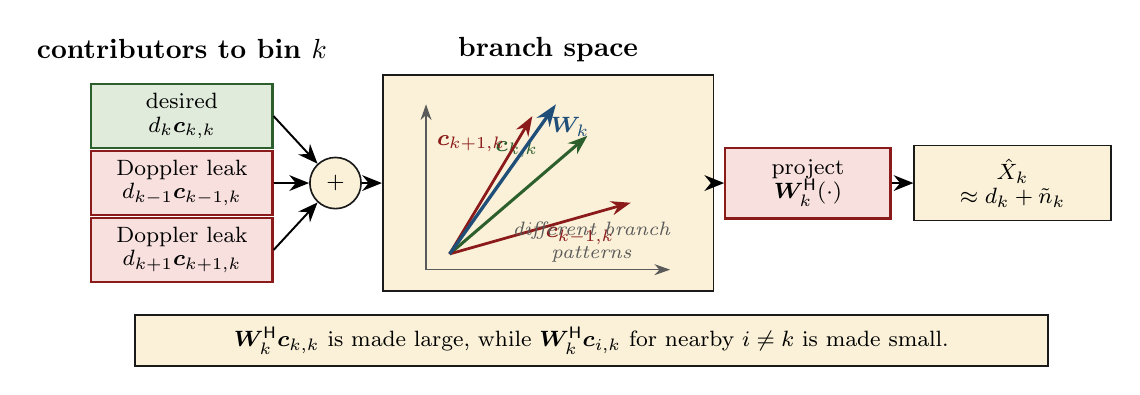
\begin{tikzpicture}[x=1cm,y=1cm,every node/.style={font=\footnotesize}]
    % Contributors
    \node[font=\bfseries] at (-5.2,1.75) {contributors to bin $k$};
    \node[draw=junagreen,fill=grnbg,line width=0.8pt,
          minimum width=2.3cm,minimum height=0.55cm,align=center] (des) at (-5.2,0.90)
      {desired\\[-1pt] $d_k\vc_{k,k}$};
    \node[draw=rpcred,fill=redbg,line width=0.8pt,
          minimum width=2.3cm,minimum height=0.55cm,align=center] (leak1) at (-5.2,0.05)
      {Doppler leak\\[-1pt] $d_{k-1}\vc_{k-1,k}$};
    \node[draw=rpcred,fill=redbg,line width=0.8pt,
          minimum width=2.3cm,minimum height=0.55cm,align=center] (leak2) at (-5.2,-0.80)
      {Doppler leak\\[-1pt] $d_{k+1}\vc_{k+1,k}$};

    \node[draw=ink,fill=paper,circle,line width=0.6pt,
          inner sep=0pt,minimum size=0.65cm] (sum) at (-3.25,0.05) {$+$};
    \draw[flowarr] (des.east) -- (sum);
    \draw[flowarr] (leak1.east) -- (sum);
    \draw[flowarr] (leak2.east) -- (sum);

    % Branch-space box
    \node[draw=ink,fill=paper,line width=0.6pt,
          minimum width=4.2cm,minimum height=2.75cm] (spacebox) at (-0.55,0.05) {};
    \node[font=\bfseries] at (-0.55,1.75) {branch space};
    \draw[flowarr] (sum.east) -- (spacebox.west);

    \begin{scope}[shift={(-0.55,0.00)}]
      \draw[color=inkgray,-{Stealth[length=2mm,width=1.4mm]},line width=0.45pt]
        (-1.55,-1.05) -- (-1.55,1.05);
      \draw[color=inkgray,-{Stealth[length=2mm,width=1.4mm]},line width=0.45pt]
        (-1.55,-1.05) -- (1.55,-1.05);

      \draw[-{Stealth[length=2.5mm,width=1.8mm]},line width=1.1pt,color=junagreen]
        (-1.25,-0.85) -- (0.50,0.65)
        node[pos=0.72,above left] {$\vc_{k,k}$};
      \draw[-{Stealth[length=2.5mm,width=1.8mm]},line width=1.0pt,color=rpcred]
        (-1.25,-0.85) -- (1.05,-0.20)
        node[pos=0.72,below] {$\vc_{k-1,k}$};
      \draw[-{Stealth[length=2.5mm,width=1.8mm]},line width=1.0pt,color=rpcred]
        (-1.25,-0.85) -- (-0.20,0.90)
        node[pos=0.80,left] {$\vc_{k+1,k}$};
      \draw[-{Stealth[length=2.8mm,width=2.0mm]},line width=1.2pt,color=boxblue]
        (-1.25,-0.85) -- (0.10,1.05)
        node[pos=0.85,right] {$\vW_k$};

      \node[font=\scriptsize\itshape\color{inkgray},align=center] at (0.55,-0.70)
        {different branch\\patterns};
    \end{scope}

    % Projection and output
    \node[draw=rpcred,fill=redbg,line width=0.8pt,
          minimum width=2.1cm,minimum height=0.9cm,align=center] (proj) at (2.75,0.05)
      {project\\[-1pt] $\vW_k^{\herm}(\cdot)$};
    \node[draw=ink,fill=paper,line width=0.6pt,
          minimum width=2.5cm,minimum height=0.95cm,align=center] (out) at (5.35,0.05)
      {$\hX_k$\\[-1pt] $\approx d_k+\tilde n_k$};
    \draw[flowarr] (spacebox.east) -- (proj.west);
    \draw[flowarr] (proj.east) -- (out.west);

    % Dot-product interpretation
    \node[draw=ink,line width=0.6pt,fill=paper,
          minimum width=11.6cm,minimum height=0.65cm,
          align=center,inner sep=4pt] at (0,-1.95)
      {$\vW_k^{\herm}\vc_{k,k}$ is made large, while
       $\vW_k^{\herm}\vc_{i,k}$ for nearby $i\ne k$ is made small.};
  \end{tikzpicture}
  \end{center}

\end{frame}

% =====================================================================
%  Slide 7: Normal Equations and RLS
% =====================================================================
\begin{frame}{6. Normal equations}

  \begin{columns}[T,onlytextwidth]
    \begin{column}{0.50\textwidth}
      \begin{itemize}\setlength{\itemsep}{0.35em}
        \item Choose $\vW_k$ so $\vW_k^{\herm}\vY_p$ matches the known pilot $X_p$
        \item Stack pilot branch vectors as rows:
      \end{itemize}
      \vspace{-0.5em}
      \[
        \bm U_k=
        \begin{bmatrix}
          \vY_{p_1}^{\herm}\\[-1pt]
          \vdots\\[-1pt]
          \vY_{p_P}^{\herm}
        \end{bmatrix},
        \qquad
        \bm d_k=
        \begin{bmatrix}
          X_{p_1}\\[-1pt]
          \vdots\\[-1pt]
          X_{p_P}
        \end{bmatrix}.
      \]
    \end{column}

    \begin{column}{0.48\textwidth}
      \vspace{-0.3em}
      \[
        \min_{\vW_k}\;
        \|\bm U_k\vW_k-\bm d_k\|_2^2
        +\delta\|\vW_k\|_2^2
      \]
      \vspace{-0.5em}
      \[
        (\bm U_k^{\herm}\bm U_k+\delta\bm I)\vW_k
        =
        \bm U_k^{\herm}\bm d_k
      \]
      \vspace{-0.5em}
      \[
        \widehat{\vW}_k=\bm R_k^{-1}\bm r_k.
      \]
    \end{column}
  \end{columns}

  \vfill
  \begin{center}
    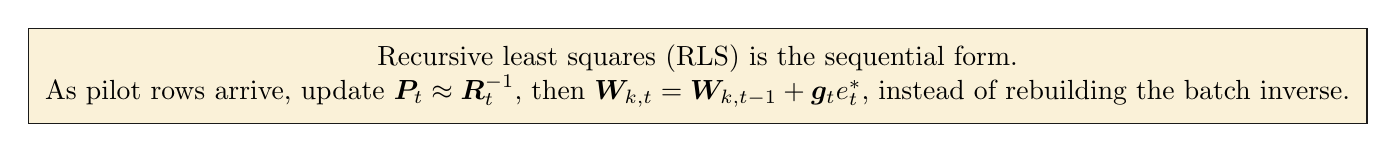
\begin{tikzpicture}
      \node[draw=ink,line width=0.6pt,fill=paper,
            minimum width=13.8cm,minimum height=1.0cm,
            align=center,inner sep=6pt]
        {Recursive least squares (RLS) is the sequential form.\\
         As pilot rows arrive, update $\bm P_t\approx\bm R_t^{-1}$, then
         $\vW_{k,t}=\vW_{k,t-1}+\bm g_t e_t^*$, instead of rebuilding the batch inverse.};
    \end{tikzpicture}
  \end{center}

\end{frame}

% =====================================================================
%  Slide 7: From the combiner to the branch model
% =====================================================================
\begin{frame}{7. Scalar or vector}

  \begin{columns}[T,onlytextwidth]
    \begin{column}{0.52\textwidth}
      \textbf{\color{rpcred}Partial-FFT combining.} Compress $\vY_k$ to one number, then decode:
      \[
        \hX_k \;=\; \vW_k^{\herm}\,\vY_k .
      \]
      Pilots train $\vW_k$; branch structure is discarded.

      \vspace{0.3em}
      \textbf{\color{junagreen}JUNA view.} Keep the $M$-vector and ask which symbols \emph{generated} it:
      \[
        \vY_k \;=\; \sum_{q\in\Bk}\vc_{k,q}\,s_q \;+\; \vn_k .
      \]
      Each $\vc_{k,q}\!\in\!\Cx^{M}$ is the leakage profile from $q$ into the $M$ branches.
    \end{column}

    \begin{column}{0.47\textwidth}
      \begin{center}
      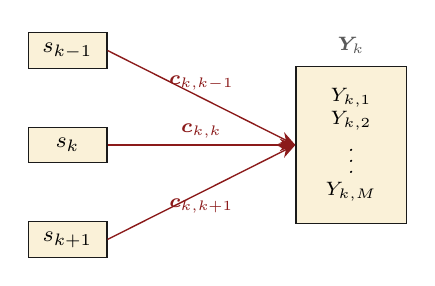
\begin{tikzpicture}[x=1cm,y=1cm,font=\footnotesize]
        \node[branchbox,minimum width=1.4cm,minimum height=2.0cm,font=\scriptsize\itshape] (br) at (3.6,0)
          {$Y_{k,1}$\\$Y_{k,2}$\\$\vdots$\\$Y_{k,M}$};
        \node[font=\scriptsize\itshape\color{inkgray},above=1pt of br] {$\vY_k$};

        \node[smallbox,minimum width=1.0cm,minimum height=0.45cm] (sa) at (0,1.2)  {$s_{k-1}$};
        \node[smallbox,minimum width=1.0cm,minimum height=0.45cm] (sb) at (0,0.0)  {$s_{k}$};
        \node[smallbox,minimum width=1.0cm,minimum height=0.45cm] (sc) at (0,-1.2) {$s_{k+1}$};

        \draw[redarr] (sa.east) -- node[above=-1pt,font=\scriptsize\itshape] {$\vc_{k,k-1}$} (br.west);
        \draw[redarr] (sb.east) -- node[above=-1pt,font=\scriptsize\itshape] {$\vc_{k,k}$}   (br.west);
        \draw[redarr] (sc.east) -- node[below=-1pt,font=\scriptsize\itshape] {$\vc_{k,k+1}$} (br.west);
      \end{tikzpicture}
      \end{center}
      \begin{center}{\scriptsize\itshape\color{inkgray}each $\vc_{k,q}$ is itself an $M$-vector}\end{center}
    \end{column}
  \end{columns}

  \begin{center}
    {\itshape\small Partial-FFT combining compresses $\vY_k$ before the code is used.\;
     JUNA models $\vY_k$ as a sum of nearby symbols times branch-domain profiles.}
  \end{center}
\end{frame}

% =====================================================================
%  Slide 8: Where the Off-Diagonal Coefficients Come From
% =====================================================================
\begin{frame}{8. Off-diagonal coefficients}

  \begin{columns}[T,onlytextwidth]
    \begin{column}{0.44\textwidth}
      \begin{itemize}\setlength{\itemsep}{0.22em}
        \item Static: only $\vc_{k,k}$ nonzero
        \item Doppler makes $H_i(t)$ \emph{vary inside} every window
        \item Each neighbor $q$ leaks into branch $m$
        \item Stack across $M$ branches $\Rightarrow$ $\vc_{k,q}\in\Cx^{M}$
        \item Leakage decays with $|k-q|$ $\Rightarrow$ \textbf{banded}
        \item Partial-FFT combining cancels these terms; JUNA \emph{models} them
      \end{itemize}
    \end{column}

    \begin{column}{0.55\textwidth}
      \begin{center}
      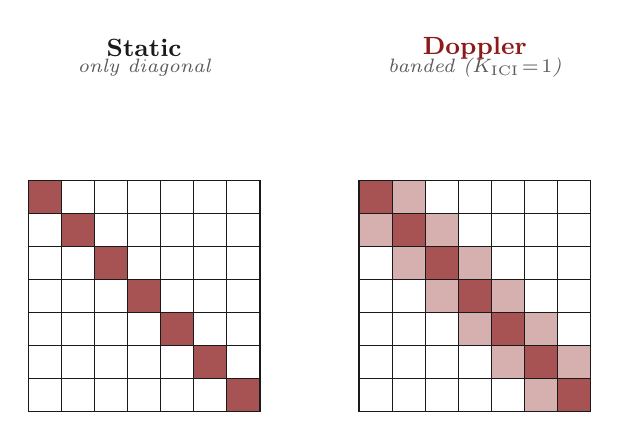
\begin{tikzpicture}[x=0.42cm,y=0.42cm,font=\footnotesize]
        \begin{scope}[shift={(0,0)}]
          \node[font=\bfseries\small\color{ink}] at (3.5,4.0) {Static};
          \node[font=\scriptsize\itshape\color{inkgray}] at (3.5,3.4) {only diagonal};
          \foreach \i in {1,...,7} {
            \fill[rpcred!75] (\i-1,-\i+1) rectangle (\i,-\i);
          }
          \draw[step=1,ink,line width=0.25pt] (0,0) grid (7,-7);
          \draw[ink,line width=0.5pt] (0,0) rectangle (7,-7);
        \end{scope}
        \begin{scope}[shift={(10,0)}]
          \node[font=\bfseries\small\color{rpcred}] at (3.5,4.0) {Doppler};
          \node[font=\scriptsize\itshape\color{inkgray}] at (3.5,3.4) {banded ($K_{\rm ICI}\!=\!1$)};
          \foreach \i in {1,...,6} {
            \fill[rpcred!35] (\i,-\i+1) rectangle (\i+1,-\i);
          }
          \foreach \i in {2,...,7} {
            \fill[rpcred!35] (\i-2,-\i+1) rectangle (\i-1,-\i);
          }
          \foreach \i in {1,...,7} {
            \fill[rpcred!75] (\i-1,-\i+1) rectangle (\i,-\i);
          }
          \draw[step=1,ink,line width=0.25pt] (0,0) grid (7,-7);
          \draw[ink,line width=0.5pt] (0,0) rectangle (7,-7);
        \end{scope}
      \end{tikzpicture}
      \end{center}
      \begin{center}{\scriptsize\itshape\color{inkgray}rows $=$ received $\vY_k$,\; columns $=$ transmitted $s_q$}\end{center}
    \end{column}
  \end{columns}
\end{frame}

% =====================================================================
%  Slide 9: The Banded Mixing Matrix Picture
% =====================================================================
\begin{frame}{9. The mixing matrix}

  Stack carriers: $\vY=[\vY_1;\dots;\vY_K]\in\Cx^{MK}$, \ $\vs=[s_1;\dots;s_K]\in\Cx^{K}$.
  Each block-row of $\vC$ is the mixing rule for one $\vY_k$; each shaded cell is itself an $M\!\times\!1$ vector.

  \vspace{0.35em}
  \begin{center}
  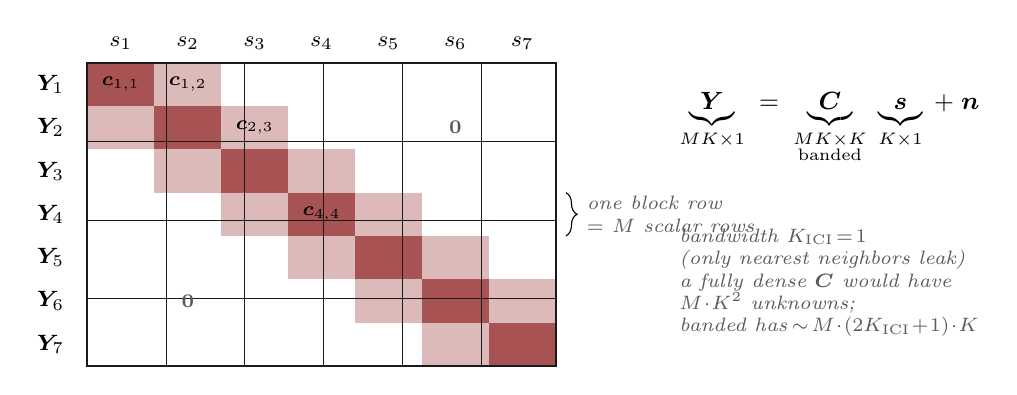
\begin{tikzpicture}[x=0.85cm,y=0.55cm,font=\footnotesize]
    % column labels (s_q)
    \foreach \q in {1,2,3,4,5,6,7} {
      \node at (\q-0.5, 0.45) {$s_{\q}$};
    }
    % row labels (Y_k)
    \foreach \k in {1,2,3,4,5,6,7} {
      \node at (-0.55, -\k+0.5) {$\vY_{\k}$};
    }
    % super & sub diagonals (lighter)
    \foreach \i in {1,2,3,4,5,6} {
      \fill[rpcred!30] (\i,-\i+1) rectangle (\i+1,-\i);
    }
    \foreach \i in {2,3,4,5,6,7} {
      \fill[rpcred!30] (\i-2,-\i+1) rectangle (\i-1,-\i);
    }
    % diagonal (darker)
    \foreach \i in {1,2,3,4,5,6,7} {
      \fill[rpcred!75] (\i-1,-\i+1) rectangle (\i,-\i);
    }
    % grid
    \draw[step=1cm,ink,line width=0.3pt] (0,0) grid (7,-7);
    \draw[ink,line width=0.7pt] (0,0) rectangle (7,-7);

    % a few example labels
    \node[font=\scriptsize] at (0.5,-0.5) {$\vc_{1,1}$};
    \node[font=\scriptsize] at (1.5,-0.5) {$\vc_{1,2}$};
    \node[font=\scriptsize] at (2.5,-1.5) {$\vc_{2,3}$};
    \node[font=\scriptsize] at (3.5,-3.5) {$\vc_{4,4}$};
    \node[font=\scriptsize\color{inkgray}] at (5.5,-1.5) {$\mathbf 0$};
    \node[font=\scriptsize\color{inkgray}] at (1.5,-5.5) {$\mathbf 0$};

    % brace for one block row showing M entries
    \draw[decorate,decoration={brace,amplitude=4pt}] (7.15,-3) -- node[right=4pt,font=\scriptsize\itshape\color{inkgray},align=left] {one block row\\$=$ $M$ scalar rows} (7.15,-4);

    % equation on right
    \node[anchor=west,font=\small] at (8.7,-1.5)
      {$\underbrace{\vY}_{MK\times 1}\;=\;\underbrace{\vC}_{\substack{MK\times K\\\text{banded}}}\;\underbrace{\vs}_{K\times 1}\;+\;\vn$};

    \node[anchor=west,font=\scriptsize\itshape\color{inkgray},align=left] at (8.7,-4.3)
      {bandwidth $K_{\rm ICI}\!=\!1$\\(only nearest neighbors leak)};
    \node[anchor=west,font=\scriptsize\itshape\color{inkgray},align=left] at (8.7,-5.6)
      {a fully dense $\vC$ would have\\$M\!\cdot\!K^2$ unknowns;\\banded has $\!\sim\! M\!\cdot\!(2K_{\rm ICI}\!+\!1)\!\cdot\!K$};
  \end{tikzpicture}
  \end{center}

  \vspace{-0.1em}
  \begin{center}
    {\itshape\small The static-OFDM model is the special case $K_{\rm ICI}\!=\!0$:
    $\vC$ collapses to a (block) diagonal and $\hX_k\!\propto\!\vc_{k,k}^{\herm}\vY_k$.}
  \end{center}
\end{frame}

% =====================================================================
%  Slide 10: Why Pilots Help
% =====================================================================
\begin{frame}{10. Pilots}

  \begin{columns}[T,onlytextwidth]
    \begin{column}{0.50\textwidth}
      The model $\vY_k=\sum_q\vc_{k,q}s_q+\vn_k$ is \emph{bilinear}:
      \[
        \vc_{k,q}\,s_q
        \;=\;
        \big(\alpha\vc_{k,q}\big)\big(\tfrac{1}{\alpha}s_q\big).
      \]
      Without anchors, scaling $\vC$ up and $\vs$ down leaves $\vY$ unchanged.

      \vspace{0.3em}
      \textbf{Pilots fix this.} On pilot column $p$, $s_p\!=\!P_p$ is \emph{known}, so
      \[
        \vc_{k,p}\,P_p \;\;\longleftarrow\;\; \text{linear in }\vc_{k,p}.
      \]
      A pilot inside row $k$'s band gives one identified $\vc_{k,p}$ and shrinks the search space for neighboring data unknowns.

      \vspace{0.2em}
      Pilots also train $\vW_p^{\herm}\vY_p\!\approx\!P_p$, giving JUNA a meaningful warm start.
    \end{column}

    \begin{column}{0.49\textwidth}
      \begin{center}
      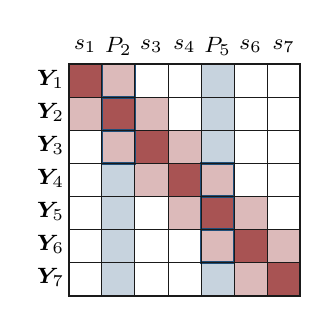
\begin{tikzpicture}[x=0.42cm,y=0.42cm,font=\footnotesize]
        \foreach \q/\lab in {1/{$s_1$},2/{$\!P_2\!$},3/{$s_3$},4/{$s_4$},5/{$\!P_5\!$},6/{$s_6$},7/{$s_7$}} {
          \node at (\q-0.5, 0.55) {\lab};
        }
        \foreach \q in {2,5} {
          \fill[boxblue!25] (\q-1,0) rectangle (\q,-7);
        }
        \foreach \i in {1,2,3,4,5,6} {
          \fill[rpcred!30] (\i,-\i+1) rectangle (\i+1,-\i);
        }
        \foreach \i in {2,3,4,5,6,7} {
          \fill[rpcred!30] (\i-2,-\i+1) rectangle (\i-1,-\i);
        }
        \foreach \i in {1,2,3,4,5,6,7} {
          \fill[rpcred!75] (\i-1,-\i+1) rectangle (\i,-\i);
        }
        % outline pilot-band intersections
        \draw[boxblue,line width=0.9pt] (1,0) rectangle (2,-1);
        \draw[boxblue,line width=0.9pt] (1,-1) rectangle (2,-2);
        \draw[boxblue,line width=0.9pt] (1,-2) rectangle (2,-3);
        \draw[boxblue,line width=0.9pt] (4,-3) rectangle (5,-4);
        \draw[boxblue,line width=0.9pt] (4,-4) rectangle (5,-5);
        \draw[boxblue,line width=0.9pt] (4,-5) rectangle (5,-6);

        \draw[step=1,ink,line width=0.3pt] (0,0) grid (7,-7);
        \draw[ink,line width=0.6pt] (0,0) rectangle (7,-7);

        \foreach \k in {1,2,3,4,5,6,7} {
          \node at (-0.55, -\k+0.55) {$\vY_{\k}$};
        }
      \end{tikzpicture}
      \end{center}
      \begin{center}
        {\scriptsize\itshape\color{inkgray}blue columns: pilots\quad blue outlines: linear in $\vc_{k,p}$}
      \end{center}
    \end{column}
  \end{columns}
\end{frame}

% =====================================================================
%  Slide 11: The JUNA Objective
% =====================================================================
\begin{frame}{11. The JUNA Objective}
\framesubtitle{one cost over $(\vC,\vW,\vz)$ --- six jobs in one place}

  \vspace{-0.25em}
  \[
    \mathcal A_k(\vC,\vz)=\sum_{q\in\Bk}\vc_{k,q}s_q(\vz),\qquad
    \hX_k=\vW_k^{\herm}\vY_k,\qquad
    s_k(\vz)=\tfrac{1}{\sqrt 2}\big(\tanh z_{i_1}+j\tanh z_{i_2}\big).
  \]

  \vspace{-0.6em}
  {\scriptsize
  \[
  \begin{aligned}
  \mathcal L(\vC,\vW,\vz)
  &=
  \underbrace{\lambda_d\sum_{k\in\mathcal K}
    \big\|\vY_k-\sum_{q\in\Bk}\vc_{k,q}s_q(\vz)\big\|_{\Sigma_k^{-1}}^2}_{\textstyle\textcolor{rpcred}{\text{(A) branch-model fit}}}
  \;+\;
  \underbrace{\eta\sum_{p\in\mathcal P}\big|\vW_p^{\herm}\vY_p-P_p\big|^2}_{\textstyle\textcolor{boxblue}{\text{(B) pilot anchor}}}
  \;+\;
  \underbrace{\rho\sum_{k\in\mathcal D}\big|\vW_k^{\herm}\vY_k-s_k(\vz)\big|^2}_{\textstyle\textcolor{boxblue}{\text{(C) combiner--symbol tie}}}
  \\[-0.3em]
  &\quad+\;
  \underbrace{\gamma_C\|\vC\|_F^2+\gamma_W\sum_k\|\vW_k\|_2^2}_{\textstyle\textcolor{inkgray}{\text{(D) ridge}}}
  \;+\;
  \underbrace{\gamma_S\sum_k\|\vW_{k+1}-\vW_k\|_2^2}_{\textstyle\textcolor{inkgray}{\text{(E) frequency smoothness}}}
  \;+\;
  \underbrace{\lambda_p\,\mathcal R_{\rm par}(\vz)}_{\textstyle\textcolor{junagreen}{\text{(F) LDPC parity}}} .
  \end{aligned}
  \]
  }

  \vspace{-0.2em}
  \begin{center}
  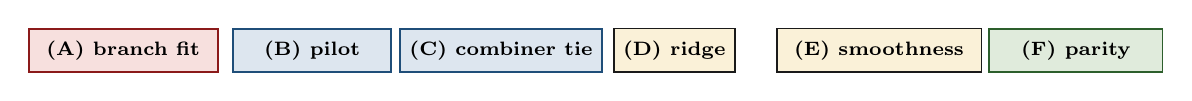
\begin{tikzpicture}[x=1cm,y=1cm,font=\scriptsize]
    \node[draw=rpcred,fill=redbg,line width=0.7pt,minimum width=2.4cm,minimum height=0.55cm,align=center,font=\scriptsize\bfseries] at (-6.0,0) {(A) branch fit};
    \node[draw=boxblue,fill=blubg,line width=0.7pt,minimum width=2.0cm,minimum height=0.55cm,align=center,font=\scriptsize\bfseries] at (-3.6,0) {(B) pilot};
    \node[draw=boxblue,fill=blubg,line width=0.7pt,minimum width=2.4cm,minimum height=0.55cm,align=center,font=\scriptsize\bfseries] at (-1.2,0) {(C) combiner tie};
    \node[draw=ink,fill=paper,line width=0.6pt,minimum width=1.5cm,minimum height=0.55cm,align=center,font=\scriptsize\bfseries] at ( 1.0,0) {(D) ridge};
    \node[draw=ink,fill=paper,line width=0.6pt,minimum width=2.6cm,minimum height=0.55cm,align=center,font=\scriptsize\bfseries] at ( 3.6,0) {(E) smoothness};
    \node[draw=junagreen,fill=grnbg,line width=0.7pt,minimum width=2.2cm,minimum height=0.55cm,align=center,font=\scriptsize\bfseries] at ( 6.1,0) {(F) parity};
  \end{tikzpicture}
  \end{center}

  \begin{center}
    {\itshape\small Three unknowns $(\vC,\vW,\vz)$, six terms; pilots, code, and branch model regularize one another.}
  \end{center}
\end{frame}

% =====================================================================
%  Slide 12: What Each Term Buys + Relation to RPC
% =====================================================================
\begin{frame}{12. The six terms}

  \renewcommand{\arraystretch}{1.20}
  \arrayrulecolor{ink}
  \scriptsize
  \begin{center}
  \begin{tabular}{|>{\columncolor{labelbg}\bfseries\footnotesize}p{2.5cm}
                  |>{\columncolor{paper}}p{4.5cm}
                  |>{\columncolor{paper}}p{6.4cm}|}
    \hline
    \rowcolor{headerbg}
    \multicolumn{1}{|c|}{\bfseries Term}
      & \multicolumn{1}{c|}{\bfseries What it forces}
      & \multicolumn{1}{c|}{\bfseries Why you need it} \\
    \hline
    \textcolor{rpcred}{(A) branch fit}
      & $\vY_k\!\approx\!\sum_q\vc_{k,q}s_q(\vz)$ on \emph{every} carrier
      & Uses all $K$ block rows of $\vC$, not just pilot rows. Couples $\vC$ to $\vz$ so reliable data symbols become ``soft pilots''. \\
    \hline
    \textcolor{boxblue}{(B) pilot anchor}
      & $\vW_p^{\herm}\vY_p\!\approx\!P_p$
      & The classical Partial-FFT training cost. Pins $\vW_p$ to known targets, and (via the bilinear coupling) helps identify $\vc_{k,p}$. \\
    \hline
    \textcolor{boxblue}{(C) combiner tie}
      & $\vW_k^{\herm}\vY_k\!\approx\!s_k(\vz)$ on data carriers
      & Decision direction \emph{inside} the loop: data carriers act like additional pilots once $\vz$ is partly trusted. \\
    \hline
    \textcolor{ink}{(D) ridge}
      & $\|\vC\|_F^2$, $\|\vW_k\|_2^2$ small
      & Stabilizes ill-conditioned inverses (sparse pilots, banded but high-dimensional $\vC$). \\
    \hline
    \textcolor{ink}{(E) smoothness}
      & $\vW_{k+1}\!\approx\!\vW_k$
      & Doppler-induced ICI varies smoothly with $k$. Borrows strength across neighboring carriers. \\
    \hline
    \textcolor{junagreen}{(F) parity}
      & $\prod_{i\in\mathcal N_j}\!\xi_i(\vz)\!\to\!+1$
      & Lets the low-density parity-check (LDPC) code shape the front end --- not only the post-detector. Where pilots run out, parity provides anchoring. \\
    \hline
  \end{tabular}
  \end{center}

  \vspace{0.25em}
  \begin{center}
    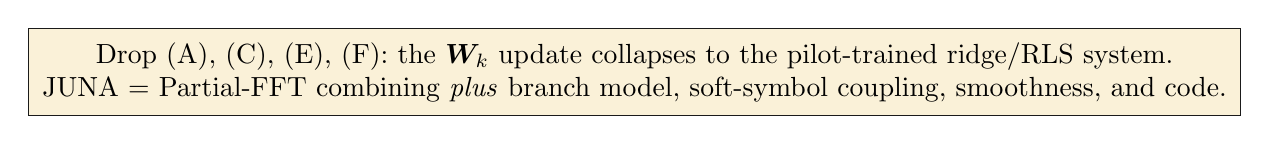
\begin{tikzpicture}
      \node[draw=ink,fill=paper,line width=0.6pt,minimum width=14cm,minimum height=0.95cm,align=center,inner sep=5pt]
        {Drop (A), (C), (E), (F): the $\vW_k$ update collapses to the pilot-trained ridge/RLS system.\\
         JUNA $=$ Partial-FFT combining \emph{plus} branch model, soft-symbol coupling, smoothness, and code.};
    \end{tikzpicture}
  \end{center}
\end{frame}

% =====================================================================
%  Slide 11: Alternating Solver
% =====================================================================
\begin{frame}{13. Alternating Solver}

  \vspace{0.2em}
  \begin{center}
  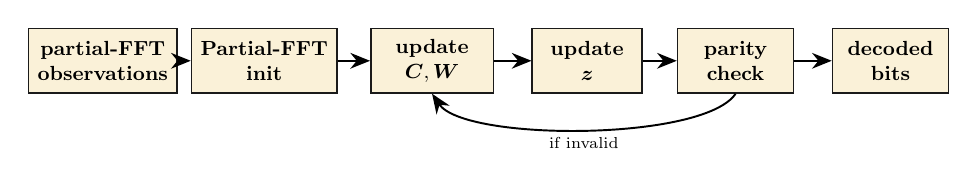
\begin{tikzpicture}[x=1cm,y=1cm,scale=0.82,every node/.style={transform shape}]
    \node[flowbox,minimum width=2.0cm] (obs) at (-6.3,0) {partial-FFT\\observations};
    \node[flowbox,minimum width=1.8cm] (init) at (-3.8,0) {Partial-FFT\\init};
    \node[flowbox,minimum width=1.9cm] (cw) at (-1.2,0) {update\\$\vC,\vW$};
    \node[flowbox,minimum width=1.7cm] (z) at (1.2,0) {update\\$\vz$};
    \node[flowbox,minimum width=1.8cm] (par) at (3.5,0) {parity\\check};
    \node[flowbox,minimum width=1.8cm] (bits) at (5.9,0) {decoded\\bits};

    \draw[flowarr] (obs.east) -- (init.west);
    \draw[flowarr] (init.east) -- (cw.west);
    \draw[flowarr] (cw.east) -- (z.west);
    \draw[flowarr] (z.east) -- (par.west);
    \draw[flowarr] (par.east) -- (bits.west);
    \draw[-{Stealth[length=2.5mm,width=2mm]},line width=0.7pt]
      (par.south) .. controls (3.0,-1.25) and (-0.7,-1.25) .. node[below,font=\scriptsize] {if invalid} (cw.south);
  \end{tikzpicture}
  \end{center}

  \vspace{0.25em}
  \begin{columns}[T,onlytextwidth]
    \begin{column}{0.49\textwidth}
      \begin{itemize}\setlength{\itemsep}{0.35em}
        \item Fixed $\vz$: update $\vC$ by ridge least squares on the branch model.
        \item Fixed $(\vC,\vz)$: update each $\vW_k$ by ridge least squares,
              plus smoothness if used.
      \end{itemize}
    \end{column}
    \begin{column}{0.49\textwidth}
      \begin{itemize}\setlength{\itemsep}{0.35em}
        \item Fixed $(\vC,\vW)$: update $\vz$ with smooth local refinement.
        \item Stop on valid parity check, stalled residual/loss, or iteration budget.
      \end{itemize}
    \end{column}
  \end{columns}

\end{frame}

% =====================================================================
%  Slide 12: Key Difference at a Glance
% =====================================================================
\begin{frame}{14. Comparison}

  \vspace{0.3em}
  \renewcommand{\arraystretch}{1.35}
  \arrayrulecolor{ink}
  \small
  \begin{center}
  \begin{tabular}{|>{\columncolor{labelbg}\bfseries}p{2.7cm}
                  |>{\columncolor{paper}}p{4.0cm}
                  |>{\columncolor{paper}}p{6.0cm}|}
    \hline
    \rowcolor{headerbg}
    \multicolumn{1}{|c|}{\bfseries Aspect}
      & \multicolumn{1}{c|}{\bfseries\color{rpcred} Partial-FFT}
      & \multicolumn{1}{c|}{\bfseries\color{junagreen} JUNA} \\
    \hline
    Model in use
      & Section II partial-FFT scalar combiner
      & Local vector model in partial-FFT (branch-domain) \\
    \hline
    What is estimated
      & Combining weights $\vW_k$
      & $\vc_{k,q}$ (for $q\in\Bk$),\ $\vW_k$,\ and $\vz_k$ \\
    \hline
    Code use
      & External to Partial-FFT combining; after scalarization
      & During estimation (coupled) \\
    \hline
    Information used
      & Only through $\hX_k$ (1 number / carrier)
      & Full vector observations and their structure \\
    \hline
    Effect
      & Information loss under residual Doppler
      & Uses local ICI and code constraints jointly \\
    \hline
  \end{tabular}
  \end{center}

\end{frame}

% =====================================================================
%  Slide 13: Why Does This Matter?
% =====================================================================
\begin{frame}{15. Data processing inequality}
\framesubtitle{(Information-Theoretic View)}

  \begin{itemize}\setlength{\itemsep}{0.25em}
    \item Partial-FFT combining forms $\hX = g(\vY)$, then decodes
    \item This induces the Markov chain:
  \end{itemize}

  \vspace{0.2em}
  \begin{center}
  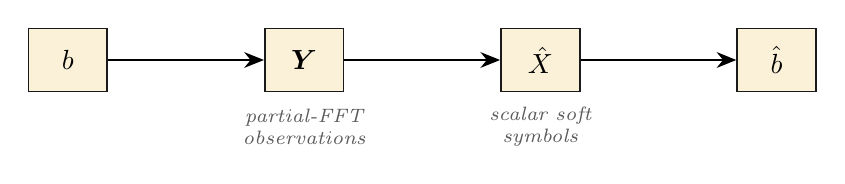
\begin{tikzpicture}[x=1cm,y=1cm]
    \node[draw=ink,fill=paper,line width=0.6pt,minimum width=1.0cm,minimum height=0.8cm] (b)  at (0,0) {$b$};
    \node[draw=ink,fill=paper,line width=0.6pt,minimum width=1.0cm,minimum height=0.8cm] (Y)  at (3.0,0) {$\vY$};
    \node[draw=ink,fill=paper,line width=0.6pt,minimum width=1.0cm,minimum height=0.8cm] (Xh) at (6.0,0) {$\hX$};
    \node[draw=ink,fill=paper,line width=0.6pt,minimum width=1.0cm,minimum height=0.8cm] (bh) at (9.0,0) {$\hb$};

    \draw[flowarr] (b.east)  -- (Y.west);
    \draw[flowarr] (Y.east)  -- (Xh.west);
    \draw[flowarr] (Xh.east) -- (bh.west);

    \node[font=\scriptsize\itshape\color{inkgray},align=center] at (3.0,-0.85) {partial-FFT\\observations};
    \node[font=\scriptsize\itshape\color{inkgray},align=center] at (6.0,-0.85) {scalar soft\\symbols};
  \end{tikzpicture}
  \end{center}

  \vspace{0.2em}
  \begin{itemize}
    \item By Data Processing Inequality:
  \end{itemize}

  \vspace{0.05em}
  \begin{center}
    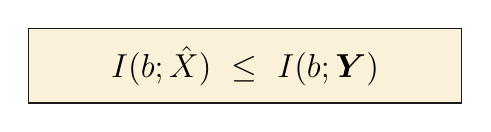
\begin{tikzpicture}
      \node[draw=ink,fill=paper,line width=0.6pt,
            minimum width=5.5cm,minimum height=0.95cm,inner sep=4pt]
        {\large $I(b;\hX)\ \le\ I(b;\vY)$};
    \end{tikzpicture}
  \end{center}

  \vspace{0.4em}
  \begin{center}
    
\begin{tikzpicture}
      \node[draw=ink,fill=paper,line width=0.6pt,
            minimum width=13cm,minimum height=1.0cm,inner sep=5pt,align=center]
        {Equality holds only if $\hX$ is sufficient for $b$ given $\vY$.\\
         Under residual Doppler (ICI), this is generally not true.};
    \end{tikzpicture}
  \end{center}
\end{frame}

% =====================================================================
%  Slide 14: Information Flow Illustration
% =====================================================================
\begin{frame}{16. Information flow}

  \vspace{0.2em}
  \begin{center}
  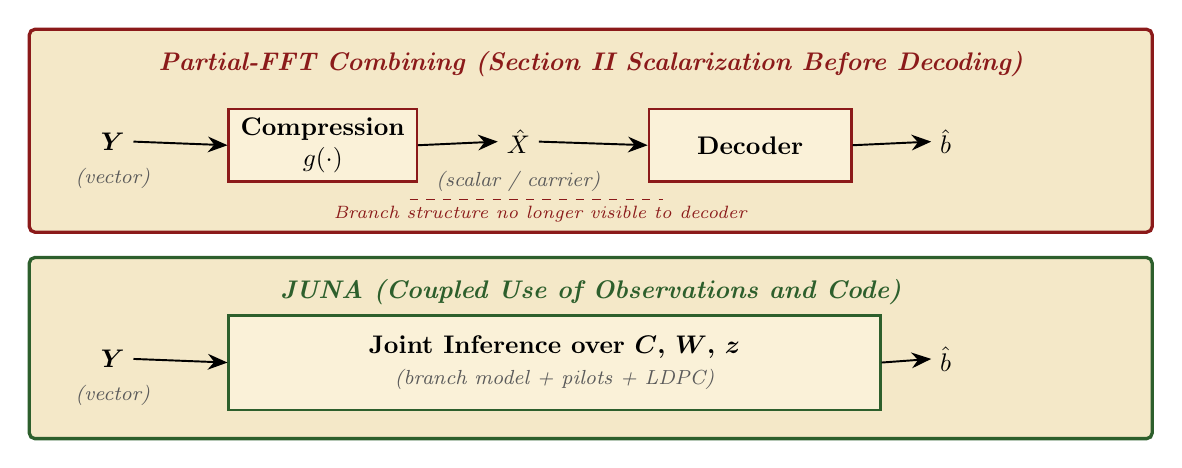
\begin{tikzpicture}[x=1cm,y=1cm,scale=0.92,every node/.style={transform shape}]
    % ----- RPC outer container (red) -----
    \node[draw=rpcred,fill=parchment,line width=1.2pt,
          minimum width=15.5cm,minimum height=2.8cm,
          rounded corners=2pt] (rpc) at (0,0) {};
    \node[font=\itshape\bfseries\color{rpcred},anchor=north]
      at ($(rpc.north)+(0,-0.2)$) {Partial-FFT Combining (Section II Scalarization Before Decoding)};

    \node[anchor=center] (Y1) at (-6.6,-0.15) {$\vY$};
    \node[anchor=north,font=\footnotesize\itshape\color{inkgray}] at (Y1.south) {(vector)};

    \node[draw=rpcred,fill=paper,line width=0.8pt,
          minimum width=2.6cm,minimum height=1.0cm,align=center] (cmp) at (-3.7,-0.2)
      {\textbf{Compression}\\$g(\cdot)$};

    \node[anchor=center] (Xh1) at (-1.0,-0.15) {$\hX$};
    \node[anchor=north,font=\footnotesize\itshape\color{inkgray}] at (Xh1.south) {(scalar / carrier)};

    \node[draw=rpcred,fill=paper,line width=0.8pt,
          minimum width=2.8cm,minimum height=1.0cm,align=center] (ldpc) at (2.2,-0.2)
      {\textbf{Decoder}};

    \node[anchor=center] (bh1) at (4.9,-0.15) {$\hb$};

    \draw[flowarr] (Y1.east)  -- (cmp.west);
    \draw[flowarr] (cmp.east) -- (Xh1.west);
    \draw[flowarr] (Xh1.east) -- (ldpc.west);
    \draw[flowarr] (ldpc.east) -- (bh1.west);

    \draw[dashed,color=rpcred,line width=0.6pt]
      (-2.5,-0.95) -- (1.0,-0.95);
    \node[font=\scriptsize\itshape\color{rpcred}] at (-0.7,-1.15)
      {Branch structure no longer visible to decoder};

    % ----- JUNA outer container (green) -----
    \node[draw=junagreen,fill=parchment,line width=1.2pt,
          minimum width=15.5cm,minimum height=2.5cm,
          rounded corners=2pt] (juna) at (0,-3.0) {};
    \node[font=\itshape\bfseries\color{junagreen},anchor=north]
      at ($(juna.north)+(0,-0.2)$) {JUNA (Coupled Use of Observations and Code)};

    \node[anchor=center] (Y2) at (-6.6,-3.15) {$\vY$};
    \node[anchor=north,font=\footnotesize\itshape\color{inkgray}] at (Y2.south) {(vector)};

    \node[draw=junagreen,fill=paper,line width=0.8pt,
          minimum width=9cm,minimum height=1.3cm,align=center] (jbox) at (-0.5,-3.2)
      {\textbf{Joint Inference over $\vC$, $\vW$, $\vz$}\\
       {\footnotesize\itshape\color{inkgray}(branch model + pilots + LDPC)}};

    \node[anchor=center] (bh2) at (4.9,-3.15) {$\hb$};

    \draw[flowarr] (Y2.east)   -- (jbox.west);
    \draw[flowarr] (jbox.east) -- (bh2.west);
  \end{tikzpicture}
  \end{center}

  \vspace{-0.3em}
  \begin{center}
    {\footnotesize\itshape\bfseries\color{junagreen}Information preserved and exploited}
  \end{center}

\end{frame}

% =====================================================================
%  Slide 15: Takeaway
% =====================================================================
\begin{frame}{17. Takeaway}

  \begin{itemize}\setlength{\itemsep}{0.35em}
    \item Partial-FFT combining splits the symbol, then combines with $\vW_k$
    \item Short intervals are closer to time-invariant
    \item Weighted combining reduces ICI before scalar detection
    \item JUNA models which nearby symbols explain the observations
    \item While scalar combining reduces ICI, it hides branch structure
    \item JUNA keeps that structure and couples it with the code
  \end{itemize}

  \vfill
  \begin{center}
    
\begin{tikzpicture}
      \node[draw=ink,fill=paper,line width=0.7pt,
            minimum width=14cm,minimum height=1.2cm,align=center,inner sep=6pt]
        {\bfseries Same observations.\quad Different use of information.\\
         \bfseries That is the fundamental difference.};
    \end{tikzpicture}
  \end{center}
  \vspace{0.3em}
\end{frame}

\end{document}
